\section{Background}
\label{section:background}

In this section, we provide the background information on automatic software repair and present an example of fixing a software vulnerability automatically.

\subsection{Automatic software repair}

The term "automatic software repair" covers many different approaches which accept a buggy program as an input and produce a fix for the target bug as an output.
In this section, we will focus only on \GV automatic repair (e.g., GenProg~\cite{le2012systematic}, SPR~\cite{long2015staged}, Prophet~\cite{long2015prophet}); we will be using the terms \GV automatic repair and automatic repair interchangeably.
The typical workflow of a \GV automatic repair tool is depicted in the Figure~\ref{figure:repair-overview}.

\begin{figure}
    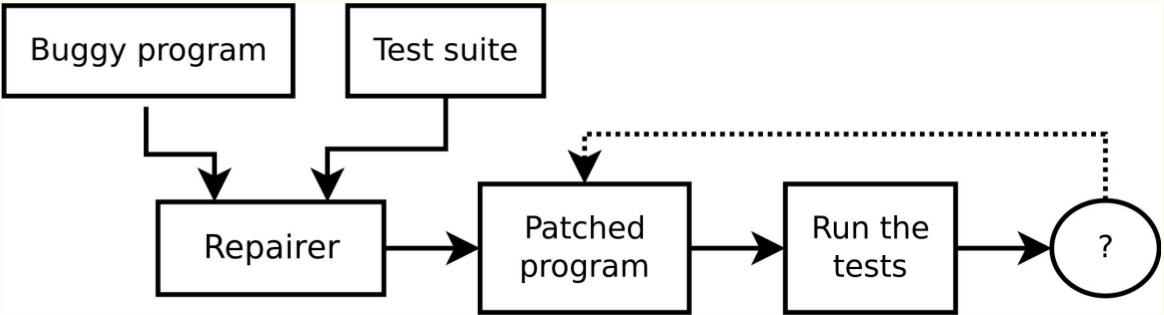
\includegraphics[width=\linewidth]{repair-overview}
    \caption{The workflow of a \GV automatic repair tool}
    \label{figure:repair-overview}
\end{figure}

Along with a buggy program, a \GV tool also accepts two types of test cases:
\begin{itemize}
    \item \textbf{Positive} test cases that verify the program's existing functionality and
    \item \textbf{Negative} test cases that expose the \emph{target} bug (i.e., the bug that the tool aims to fix)
\end{itemize}

The first step is the stage of \emph{fault localization} that produces a ranked list of statements that are suspected to be buggy. Fault localization is a well-established area of Software engineering~\cite{wong2009survey} with many different approaches; the approach adopted by most automatic repair tools is as follows: instrument each statement in the buggy program and run the program with the provided test cases. Then, based on some metric, order the statements from the most likely to be buggy to the least likely. E.g., SPR's fault localization algorithm prefers the statements that are (1) executed with more negative test cases (2) fewer positive test cases and (3) encountered later whilst executing the program with negative test cases.

After the ordered list of buggy statements is produced, the automatic repair tool applies its \emph{transformations} to attempt to fix the target bug. These transformations depend on a search space that is employed by a particular tool. To verify the correctness of the fix applied, the repairer runs all the test cases: negative ones (to verify that the bug is gone) and positive ones (to verify that no regressions are introduced). If the test cases pass, then the patch is considered to be correct and it is presented to the developer; otherwise, a repairer picks another fix from the search space and repeats the previous steps.

\subsection{GenProg}

GenProg~\cite{le2012systematic} is an automatic repair tools based on genetic programming (GP); it randomly creates candidate fixes and refines them through GP---by exchanging, adding or removing statements---until one of the fixes passes all the test cases. The main assumption that GenProg makes is that the program already has correct fixes for the target bug somewhere in the program; the goal is to find the fixes, order them properly, and apply them in the correct location. Thus, if the program does not contain ``ingredients'' for the correct fix, then the target bug cannot be repaired. In addition, Qi et al.~\cite{qi2015analysis} showed that, for the benchmarks GenProg was evaluated on, most of the fixes correspond to simple functionality deletions; they do not fix the target bug but rather just delete the functionality in which the bug resides.

\subsection{SPR} 

SPR~\cite{long2015staged} uses a notion of a so-called ``schema'', i.e., a patch template; putting different conditions into different schemas leads to a large search space with many correct patches. Contrarily to GenProg, SPR's search spaces are deterministic; SPR applies its transformations in a certain order (the order is hard-coded) until either all the test cases pass or the search space is exhausted. Next, we present the transformations in the order that SPR applies them (Figure~\ref{figure:spr-repairs} shows examples from GenProg benchmarks on which SPR was evaluated).

\textbf{Condition refinement.} Transform an existing if-condition by adding ``\texttt{\&\& P}'' or ``\texttt{|| P}''; \texttt{P} is a new condition of the form ``\texttt{(v == const)}'' or ``\texttt{(v != const)}'', where \texttt{v} is an existing variable in the current scope.
\emph{Note:} degenerate cases that either remove the whole if-block (\texttt{\&\& 0}) or always execute the if-block (\texttt{|| 1}) are possible as well.

\textbf{Condition introduction.} Transform an existing statement by adding an if-condition around it.

\textbf{Conditional control flow introduction.} Put a conditional control-flow statement (e.g., \texttt{break}, \texttt{continue}, \texttt{return}) before a statement.

\textbf{Insert initialization.} Put a call to \texttt{memset} before a statement.

\textbf{Value replacement} can either (1) replace a variable with another variable, (2) replace a function with another function that has the same signature or (3) replace a constant with another constant.

\textbf{Copy and replace}. Copy an existing statement before the target statement and apply \textbf{value replacement}.

\begin{figure}[t!]

\begin{subfigure}[b]{\linewidth}
    \lstinputlisting[language=diff]{resources/condition-refinement.diff}
    \vspace{-0.1in}
    \caption{Condition refinement from lighttpd-1913-1914}
\end{subfigure}

% libtiff-fix-tests-2e42d63ftools_tiffcrop.c-110
\begin{subfigure}[b]{\linewidth}
    \lstinputlisting[language=diff]{resources/condition-introduction.diff}
    \vspace{-0.1in}
    \caption{Condition introduction from libtiff-5b02179-3dfb33b}
\end{subfigure}

\begin{subfigure}[b]{\linewidth}
    \lstinputlisting[language=diff]{resources/conditional-control-flow.diff}
    \vspace{-0.1in}
    \caption{Conditional control-flow from php-308262-308315}
\end{subfigure}

\begin{subfigure}[b]{\linewidth}
    \lstinputlisting[language=diff]{resources/initialization.diff}
    \vspace{-0.1in}
    \caption{``Insert initialization'' from php-307846-307853}
\end{subfigure}

\begin{subfigure}[b]{\linewidth}
    \lstinputlisting[language=diff]{resources/value-replacement.diff}
    \vspace{-0.1in}
    \caption{Value replacement from php-307562-307561}
\end{subfigure}

\begin{subfigure}[b]{\linewidth}
    \lstinputlisting[language=diff]{resources/copy-and-replace.diff}
    \vspace{-0.1in}
    \caption{Copy-and-replace from php-308525-308529}
\end{subfigure}

\vspace{0.1in}
\small \caption{Examples of SPR transformations}
    \label{figure:spr-repairs}
\vspace{-0.2in}
\end{figure}

\subsection{Example of fixing a vulnerability automatically}

Next, we present an example of fixing a simple buffer overflow vulnerability automatically. In Figure~\ref{figure:example}, there is an incorrect check at line~2 with the common ``off-by-one'' mistake that leads to a value being written past the end of the buffer; line~3 shows a probable human-written fix.

Let us say that we are given a positive test case that verifies the correct value in the buffer at the index \texttt{x} (e.g., \texttt{assert(buf[x] == 0)}) and a negative test case that exposes the overflow (e.g., by making the initial value of \texttt{x} equal to \texttt{sizeof(buf)} and exposing the overflow with address sanitization\footnote{https://github.com/google/sanitizers/wiki/AddressSanitizer}).
The simplest patch that an automatic tool can generate is a mere functionality deletion; in the absence of line 5, the negative test case would stop failing; however, a positive test case would fail and reveal an incorrect fix.
Let us say that after a number of failed attempts, the repairer creates the fix shown at line 4; the positive test case passes (since \texttt{buf[x] == 0}), as well as the negative one (no overflow).
This patch is given to the developer as the correct patch and it is indeed semantically equivalent to the probable developer patch at line 3.
Note: under the SPR's transformation classification, this fix belongs to ``condition refinement'' and indeed can be potentially generated by SPR.
\begin{figure}

\lstinputlisting[language=diff]{resources/example.diff}

\vspace{0.1in}
\small \caption{Examples of SPR transformations}
    \label{figure:example}
\vspace{-0.2in}
\end{figure}

% An example:
% how about lighttpd-bug-2661-2662
% https://redmine.lighttpd.net/projects/lighttpd/repository/1?utf8=%E2%9C%93&rev=2662
% https://redmine.lighttpd.net/issues/1551
